\definecolor{azzurro}{RGB}{0, 110, 230}
\definecolor{verde}{RGB}{90, 175, 30}
\usetikzlibrary{decorations.pathmorphing, decorations.pathreplacing, arrows.meta}

\chapter{Algoritmo di Floyd Warshall}

\section{Definizione del problema}
\subsection{Istanza}
\begin{itemize}
    \item \textbf{Il DAG }$G = (V,E,w)$
    \begin{itemize}
        \item \textbf{L'inieme di vertici }$V\ t.c\ |V|=n \quad V = \{1,\dots,n\}$
        \item $E \subseteq V^2$ è l'insieme degli archi orientati
        \item \textbf{La funzione peso }$w:E \to R^+ \implies 
        w_{ij}= 
        \begin{cases}
        0 &\text{se } i=j \\
        w(i,j) &\text{se } i \not = j \land (i,j) \in E \\
        +\infty &\text{se } i \not = j \land (i,j) \not \in E 
        \end{cases}
        $
    \end{itemize}
    \item \textbf{La matrice dei pesi }$W=(w_{ij})_{i,j\in V \times V}$  di dimensione $n \times n$ che rappresenta il grafo, contiene il peso di ogni arco $(i,j)$
\end{itemize}

\subsection{Soluzione}
$\forall (i,j) \in V^2$ (il peso di) un cammino minimo (di peso minimo) dal vertice $i$ al vertice $j$

Devo calcolare $n^2$ valori, cioè $\forall (i,j)\in V^2 \ d_{ij}\to D=(d_{ij})_{(i,j) \in V^2}$, passo da $W \to D$

$\forall (i,j) \in V^2$, il \textbf{valore ottimo} cercato $d_{ij}$ coincide con il coefficiente $d_{ij}^(n)$. La matrice di output è quindi $D=D^{(n)}$

\section{Definizione del sottoproblema di dimensione $k$}
Fissato un indice $k \in \{0,1,\dots,n\}$, per ogni coppia di vertici $(i,j) \in V^2$ il sottoproblema consiste nel trovare un cammino minimo $\mathbf{P_{ij}^{(k)}}$, un cammino minimo che va dal vertice $i$ al vertice $j$ tale che:
\begin{itemize}
    \item Se $\mathbf{k=0}$, l'insieme dei possibili \textbf{vertici intermedi} è vuoto ($\emptyset$), ossia non ci sono vertici intermedi.
    
    \item Se $\mathbf{k>0}$, gli eventuali \textbf{vertici intermedi} appartengono all'insieme $\{1,2,\dots,k\}$ (non è necessario usarli tutti, ma possono essere scelti solo da questo sottoinsieme)
\end{itemize}

\section{Definizione dei coefficienti}
\subsection{$\mathbf{d_{ij}^{(k)}}$ Peso del cammino}
$d_{ij}^{(k)}$ indica il \textbf{peso del camminimo minimo} $P_{ij}^(k)$ dal vertice $i$ al vertice $j$ i cui vertici intermedi appartengono all'insieme $\{1,\dots,k\}$


\subsection{$\mathbf{\pi_{ij}^{(k)}}$ Predecessore di $\mathbf{j}$}
$\pi_{ij}^{(k)}$ indica \textbf{il predecessore di $\mathbf{j}$} lungo il camminimo minimo $P_{ij}^{(k)}$ da $i$ a $j$ con vertici intermedi in $\{1,\dots,k\}$

\section{Equazione di ricorrenza}
\subsection{Caso base $\mathbf{k=0}$}
Quando $\mathbf{k=0}$, \textbf{non sono permessi vertici intermedi} tra $i$ e $j$. L'unico cammino possibile è l'arco diretto $(i,j)$, \uline{se esiste}.

Pertanto $D^{(0)} = W$, ovvero $\forall(i,j) \in V^2$:

{
    \large

    $$
    d_{ij}^{(0)} = w_{ij} = 
    \begin{cases}
        0 & \text{se } i=j \quad (P_{ij}^{(0)} = \langle i \rangle) \\
    \end{cases} 
    $$
}

per il coefficiente del predecessore $\pi_{ij}^{(0)}$ nel caso base:
{
    \large
    $$
        \pi_{ij}^{(0)} = 
        \begin{cases}
            i & \text{se } i \not = j \land (i,j) \in E \\
            null & \text{altrimenti } (\text{se } i=j \lor (i,j) \not \in E)
        \end{cases}
    $$
}

\subsection{Passo ricorsivo $\mathbf{k>0}$}
Per calcolare il coefficiente $d_{ij}^{(k)}$ $\forall(i,j) \in V^2$ a partire dai coefficienti della matrice precedente $D^{(k-1)}$, si valutano due possibili casi per il vertice $k$ 

\begin{itemize}
    \item \textbf{Caso 1 - $\mathbf{k \in P_{ij}^{(k)}}$}\\
    $k$ non è un vertice intermedio del camminimo minimo da $i$ a $j$, il cammino minimo da $i$ a $j$ utilizza solamente vertici intermedi appartenenti aa $\{1,2,\dots,k-1\}$.

    \begin{center}
    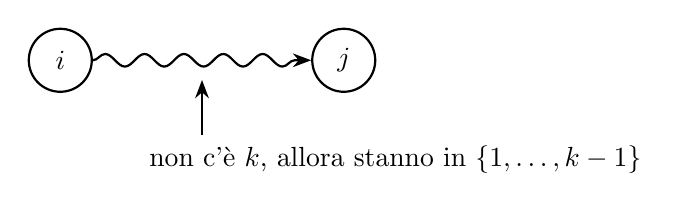
\begin{tikzpicture}[>=Stealth, thick]
        % Nodi i e j cerchiati
        \node[circle, draw, minimum size=8mm, inner sep=2pt] (i) at (0,0) {$i$};
        \node[circle, draw, minimum size=8mm, inner sep=2pt] (j) at (3.6,0) {$j$};

        % Freccia ondulata (cammino da i a j)
        \draw[->, decorate, decoration={snake, amplitude=0.8mm, segment length=5mm, post length=1.5mm}]
            (i) -- (j);

        % Freccia verticale che punta al cammino
        \draw[->] (1.8,-0.95) -- (1.8,-0.25);

        % Testo descrittivo sotto la freccia
        \node[anchor=north west] at (1.0,-0.95)
            {non c'è $k$, allora stanno in $\{1, \dots, k-1\}$};
    \end{tikzpicture}
    \end{center}

    Il suo peso ottimo è quindi già stato calcolato al passo $k-1$

    {
        \large

        $$
            d_{ij}^{(k)} = d_{ij}^{(k-1)}
        $$
    }

    \item \textbf{Caso 2 - $\mathbf{k \in P_{ij}^{(k)}}$}\\
    $k$ è un vertice intermedio del cammino minimo da $i$ a $j$, per la proprietà della sottostrutta ottima, se il cammino minimo da $i$ a $j$ passa per il vertice $k$, allora esso si scompone in due sottocammini anch'essi minimi

    \[
    \text{\textcircled{$i$}} \leadsto \text{\textcircled{$k$}} \leadsto \text{\textcircled{$j$}}
    \quad \text{posso decomporre in 2 sottocammini} \quad
    \text{\textcircled{$i$}} \overset{\textcolor{azzurro}{\in \{1, \dots, k-1\}}}{\overbrace{\leadsto\!\!\!\leadsto}} \text{\textcircled{$k$}}
    \;\text{ e }\;
    \text{\textcircled{$k$}} \overset{\textcolor{verde}{\in \{1, \dots, k-1\}}}{\overbrace{\leadsto\!\!\!\leadsto}} \text{\textcircled{$j$}}
    \]

    Il peso totale è la somma dei coefficienti dei 2 sottoproblemi

    {
        \large

        $$
        d_{ij}^{(k)} = d_{ik}^{(k-1)} + d_{kj}^{(k-1)} 
        $$
    }
\end{itemize}

Poichè non sappiamo a priori quale dei 2 casi si verifichi, li valutiamo entrambi scegliendo il minimo

{
    \large

    $$
        d_{ij}^{(k)} = \min\{d_{ij}^{(k-1)}, d_{ik}^{(k-1)} + d_{kj}^{(k-1)}\}
    $$
}

Di conseguenza, il coefficiente del predecessore $\pi_{ij}^{(k)}$ si aggiorna così

{
    \large

    $$
        \pi_{ij}^{(k)} = 
        \begin{cases}
            \pi_{ij}^{(k-1)} & \text{se } d_{ij}^{(k-1)} \leq d_{ik}^{(k-1)} + d_{kj}^{(k-1)} \quad \text{(non passo per $k$)}\\
            \pi_{ij}^{(k-1)} & \text{se } d_{ij}^{(k-1)} \geq d_{ik}^{(k-1)} + d_{kj}^{(k-1)} \quad \text{(passo per $k$)}
        \end{cases}
    $$
}

\section{Algoritmo Bottom-up}
\subsection{Pseudocodice}
L'algoritmo costruisce iterativamente le matrici $D^{(0)},D^{(1),\dots,D^{(n)}}$ di dimensione $n \times n$ fino ad ottenere $D^{(n)}$


\begin{algorithm}
    \begin{algorithmic}
        \Procedure{Calcola\_pesi\_minimi\_FW}{$V,E,W$}
            \For{$k$ from $0$ to $n$}
                \State $D^{(k)} = $ matrice di dimensione $n \times n$
            \EndFor

            \State $D^{(0)} = W$ 

            \For{$k$ from $1$ to $n$}
                \For{$i$ from $1$ to $n$}
                    \For{$j$ from $1$ to $n$}
                        \State $D^{(k)}[i,j] = D^{(k-1)}[i,j]$

                        \If{$D^{(k)}[i,j] > D^{(k-1)}[i,k] + D^{(k-1)}[k,j]$}
                            \State $D^{(k)}[i,j] = D^{(k-1)}[i,k] + D^{(k-1)}[k,j]$
                        \EndIf
                    \EndFor
                \EndFor
            \EndFor

            \State \Return $D^{(n)}$
        \EndProcedure
    \end{algorithmic}
\end{algorithm}

\subsection{Complessità}
\begin{itemize}
    \item \textbf{Complessità temporale:} $\Theta(n^3)$, poichè ci sono 3 cicli for innestati e ciascuno va da 1 a $n$, eseguendo operazioni di costo costante $O(1)$ per ogni cella
    \item \textbf{Complessità spaziale:} $O(n^2)$, perchè ogni passo $k$, per calcolare la nuova matrice $D^{(k)}$, è sufficiente tenere in memoria soltanto la matrice immediatamente precedente $D^{(k-1)}$ (servono quindi solo $2$ matrici di dimensione $n \times n$)
\end{itemize}

\section{Ricostruzione della soluzione}
Una volta calcolate le matrici fino a $k=n$, per ricostruire e stampare la sequenza di vertici del cammino minimo da $i$ a $j$ si utilizza una procedura ricorsiva sulla matrice dei predecessori $\Pi^{(N)}$

\begin{algorithm}
    \begin{algorithmic}
        \Procedure{Print-Path}{$\Pi,i,j$}
            \If{$i=j$}
                \State print($i$)

                \Else
                    \If{$\pi_{ij} \not = null$}
                        \State print(j)

                        \Else
                        \State print("$\not \exists$ cammino da $i$ a $j$")
                    \EndIf
            \EndIf
        \EndProcedure
    \end{algorithmic}
\end{algorithm}